\chapter{Results}
\label{chap:results}

\section{Introduction}

In the previous section, we presented limitations on the parameters of a commercial optical communication system that would limit the distortion on a frequency signal located on the interstices of two data channels in a DWDM scheme. The result was a phase distortion due to cross-talk (XPM) in the form
%
\begin{equation}
\phi(z,T) = 4\gamma\int_0^z |u_d(0, T-d\zeta)|^2 d\zeta.
\end{equation}
%
This shows that the phase distortion is dependent on the length of fiber, the relative velocity difference between the frequency signal and the data channels, and the power of the data channel while it changes over the course of its propagation. We can now vary these parameters and investigate their affect on the frequency stability of the frequency signal.

We choose values for the data channel power and Kerr nonlinearity $\gamma$ that resemble commercial optical communication systems, these values are used in those systems to avoid nonlinear distortions. This removes the nonlinear term in eq.~\ref{eq:simpleddata} and the data channel can be solved in the Fourier domain,
%
\begin{equation} \label{eq:datasol}
u_d(0,T-zd) = \mathcal{F}^{-1} \left\{ U_d(0, \omega)\exp\left(-\frac{\alpha}{2} z + jd\omega z + \frac{j}{2}\beta_2\omega^2z\right) \right\}
\end{equation}
%
where $\mathcal{F}^{-1}$ is the inverse Fourier transform and $U_d$ is the Fourier spectrum of the data channel.

We begin by investigating the distribution of the power of the data channel, $|u_d|^2$, as a function of length, $z$. The pulses of the data channel change over the length due to dispersion, self-phase modulation, and attenuation. The length of the fiber is chosen so that we can simulate the dispersive effects and neglect the nonlinear effects. We first simulate without attenuation to emphasize the pulse shape due to spreading. Then attenuation is added. Next we change the group velocity difference. Then we vary the data channel powers.

\section{Simulation Parameters}

The simulation data signal is a $2^{10}-1$ pseudorandom binary string that is on-off key modulated with optical power of $1$ mW with periodic boundary conditions. The fiber has an attenuation of $0.2$ dB/km, group velocity dispersion $\beta_2 = -22$ ps$^2$/km, and Kerr nonlinearity $1.3$ W$^{-1}$km$^{-1}$. The data channel has a center wavelength of $1530.0413$ nm with group velocity difference $d = 1.003$ ps/km relative to the frequency signal. Some of these parameters will vary in the following sections as we study the changes in the XPM induced phase distortion.


\section{Without Attenuation}

Neglect attenuation for the moment to evaluate the evolution of the data channel due to the material dispersion and how it affects the phase stability.

During propagation, each pulse in the data signal is going to spread outside of its bit window into its neighbors. After some long distance, the energy in each pulse will spread evenly amongst every bit. Therefore, the variance of the data signal's optical power will approach a limit as a function of fiber length.
%
\begin{figure}[htb]
	\centering
	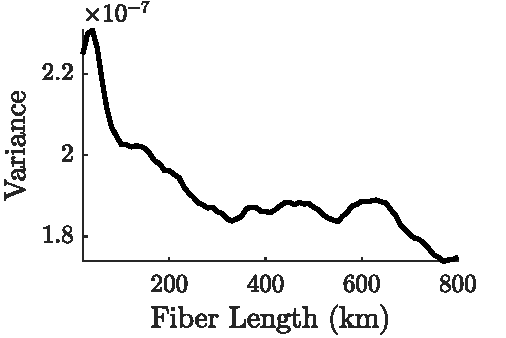
\includegraphics{img/NACalcVar}
	\caption{Data channel optical power variance vs. fiber length} \label{fig:NACalcVar}
\end{figure}
%
Figure~\ref{fig:NACalcVar} shows the data channel power variance over the fiber length of interest, we have not achieved the limit but there is not an appreciable change beyond $800$ km. Since the loss is turned off, the mean of the data channel power is fixed, and the range of the variance shows that the data channel power doesn't become significantly larger than the mean. This is important because the power will be directly related to the amount of cross-talk.

The phase error $\phi$ clearly grows as a function of distance because at every propagation length the two channels have some cross-talk which keeps accumulating. Figures \ref{fig:NAPhiMean}a and \ref{fig:NAPhiVar}b show the mean and variance of the phase distortion due to XPM respectively.
%
\begin{figure}[htb]
	\begin{tabular}{c c}
		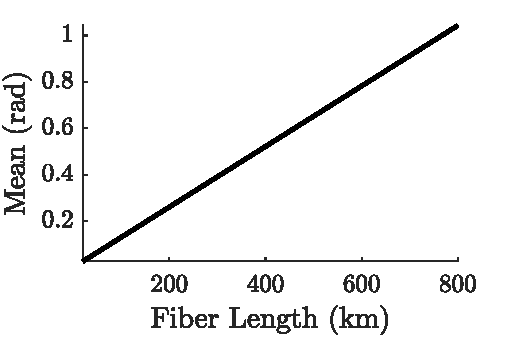
\includegraphics[width=0.5\linewidth]{img/NAPhiMean} & 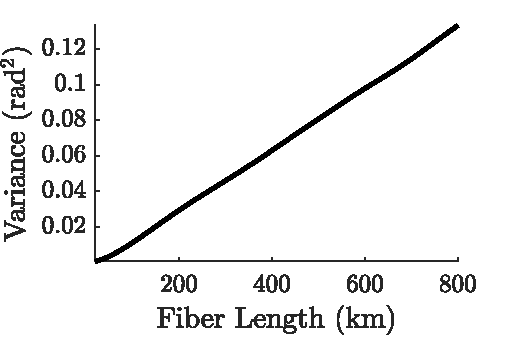
\includegraphics[width=0.5\linewidth]{img/NAPhiVar} \\
		(a) & (b)
	\end{tabular}
	\caption{(a)\label{fig:NAPhiMean} Mean of $\phi$ vs. fiber length (b)\label{fig:NAPhiVar} Variance of $\phi$ vs. fiber length}
\end{figure}
%
The mean of $\phi$ grows linearly with respect to the fiber length because without a loss mechanism the average energy in the data channel is constant. This signifies a mean additive phase error that can be compensated.

At this point we want to quantify the phase stability using measures from chapter \ref{chap:time_stability}. We first consider the first structure equation, $D^{(1)}_\phi = \langle [\phi(t+\tau) - \phi(t)]^2 \rangle$, which represents the mean phase accumulation. The structure functions are related to the autocorrelation. A typical data transmission will be a collection of random bits that are uncorrelated with eachother. As the data signal propagates through the fiber, every pulse that represents a bit will spread into its neighbors, thus the amount of time where a bit is correlated with itself increases. Figure \ref{fig:NAPhaseStability} shows $D^{(1)}_\phi$ at different lengths and agrees with this explanation. 
%
\begin{figure}[htb]
	\centering
	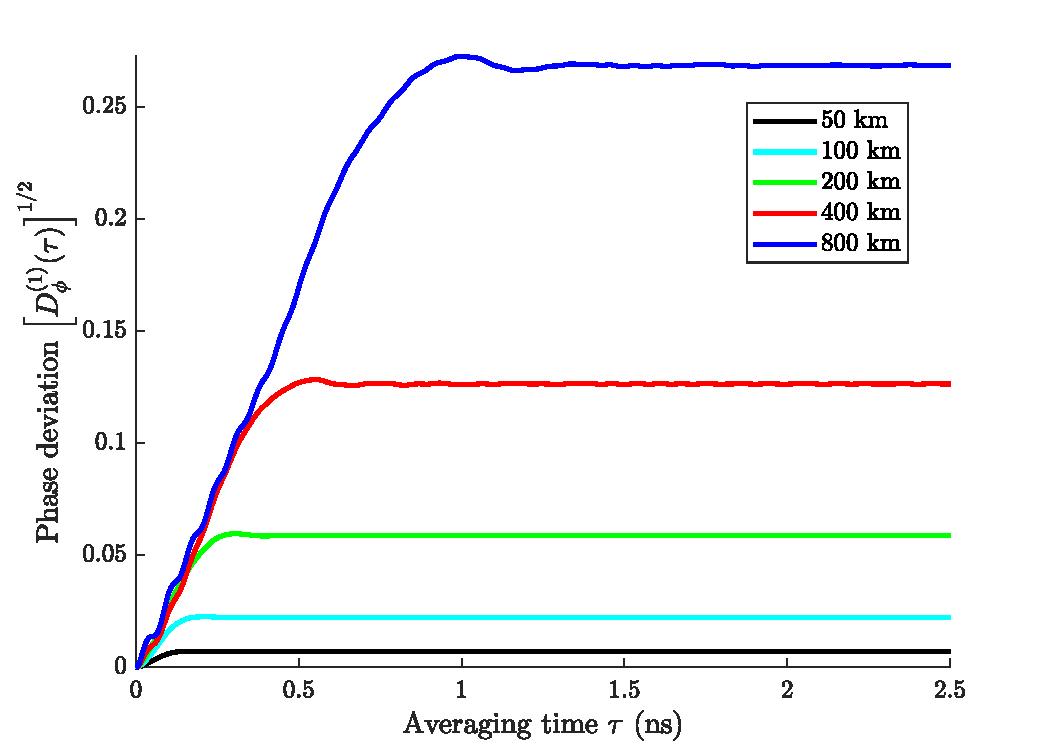
\includegraphics{img/NAPhaseStability}
	\caption{Phase Stability vs. averaging time $\tau$} \label{fig:NAPhaseStability}
\end{figure}
%
The phase stabilizes after a short amount of time.

Figure \ref{fig:NAAllanDev} shows the Allan Deviation. After a short amount of time, the short term frequency errors are averaged out at the peak, then the Allan Deviation drops off at the rate of $\tau^{-1}$. The Allan Deviation will continue this trend, because there are no long term frequency errors from the XPM. We have compute over a short time interval due to memory limitations, but we can use a linear fit for the $\tau^{-1}$ region to determine the Allan Deviation for usual averaging times. At $\tau = 1$ s ADEV $= 3\times 10^{-15}$, and at $\tau=10^3$ s ADEV $= 3\times 10^{-18}$.
%
\begin{figure}[htb]
	\centering
	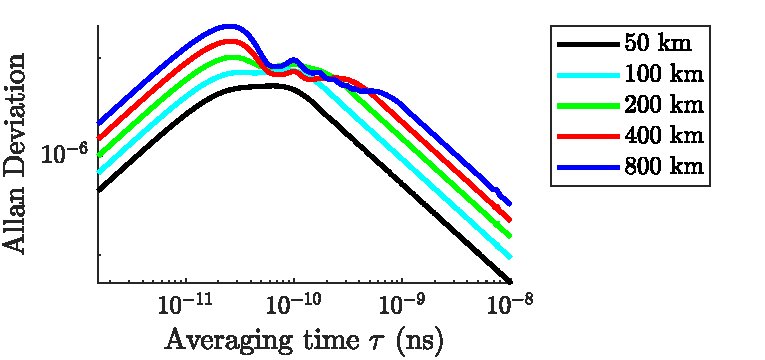
\includegraphics{img/NAAllanDev}
	\caption{Allan Deviation} \label{fig:NAAllanDev}
\end{figure}
%


\section{With Attenuation}

We now add attenuation to the data channel. We expect the results to be bounded above by the phase and frequency stability without attenuation because the effective length before the nonlinearity becomes negligible is $20$ km after each amplifier, meaning the cross-talk weakens over a quarter length between amplifiers.

%
\begin{figure}[htb]
	\centering
	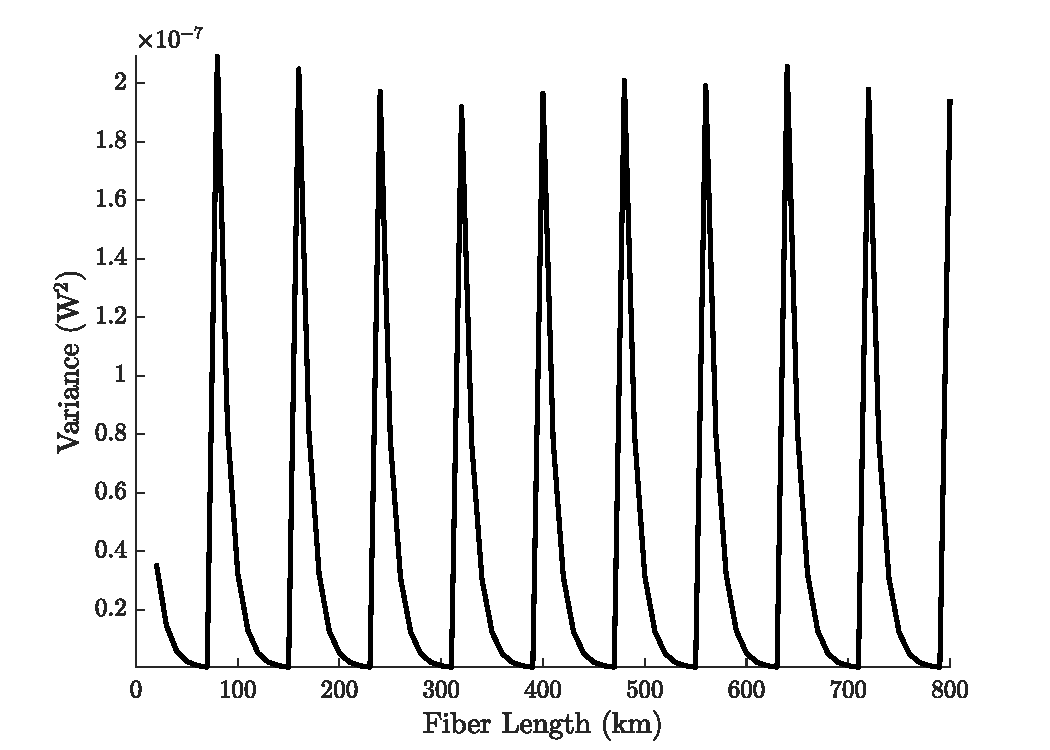
\includegraphics{img/ACalcVar}
	\caption{Data channel optical power variance vs. fiber length} \label{fig:ACalcVar}
\end{figure}
%
First, we compare the variance of the attenuated data channel with the previous section's. Figure~\ref{fig:ACalcVar} shows the data channel's optical power variance. The spikes occur every $80$ km corresponding with the amplifiers location, the spikes will grow at distances beyond $800$ km because the ASE noise will start accumulating.

The mean and variance of $\phi$ must also grow over the distance of the fiber, but there are lengths of the fiber which the power is low, so there will be steps. Figures \ref{fig:APhiMean}a and \ref{fig:APhiVar} show the mean and variance of $\phi$ respectively and show the steps where the data channel power is low. The mean and variance are less than those of the previous section.
%
\begin{figure}[htb]
	\begin{tabular}{c c}
		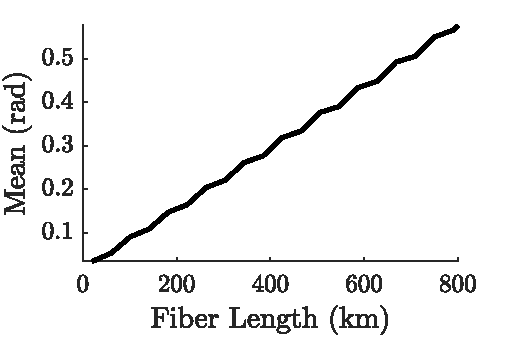
\includegraphics[width=0.5\linewidth]{img/APhiMean} & 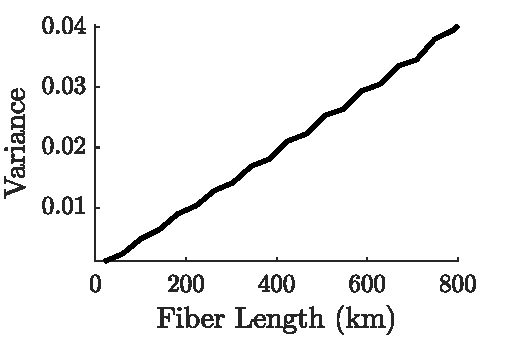
\includegraphics[width=0.5\linewidth]{img/APhiVar} \\
		(a) & (b)
	\end{tabular}
	\caption{(a)\label{fig:APhiMean} Mean of $\phi$ vs. fiber length (b)\label{fig:APhiVar} Variance of $\phi$ vs. fiber length}
\end{figure}
%

The phase stability computed as the structure function $D^{(1)}_\phi$ will asymptote like in the previous section. Since this depends on the pulse spreading due to dispersion, the asymptotes occur at the same times. However, the phase stability will be less due to attenuation. Figure~\ref{fig:APhaseStability} shows $D^{(1)}_\phi$ for different fiber lengths and agrees with the previous explanation.
%
\begin{figure}[htb]
	\centering
	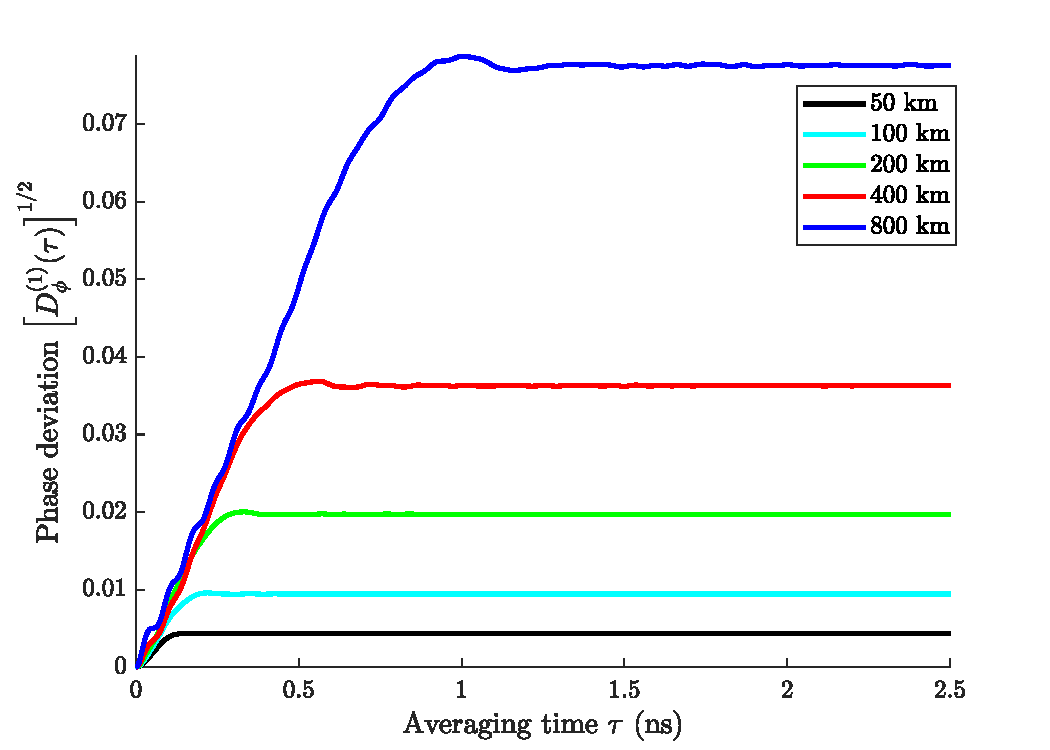
\includegraphics{img/APhaseStability}
	\caption{Phase stability with attenuation} \label{fig:APhaseStability}
\end{figure}
%

%
\begin{figure}[htb]
	\centering
	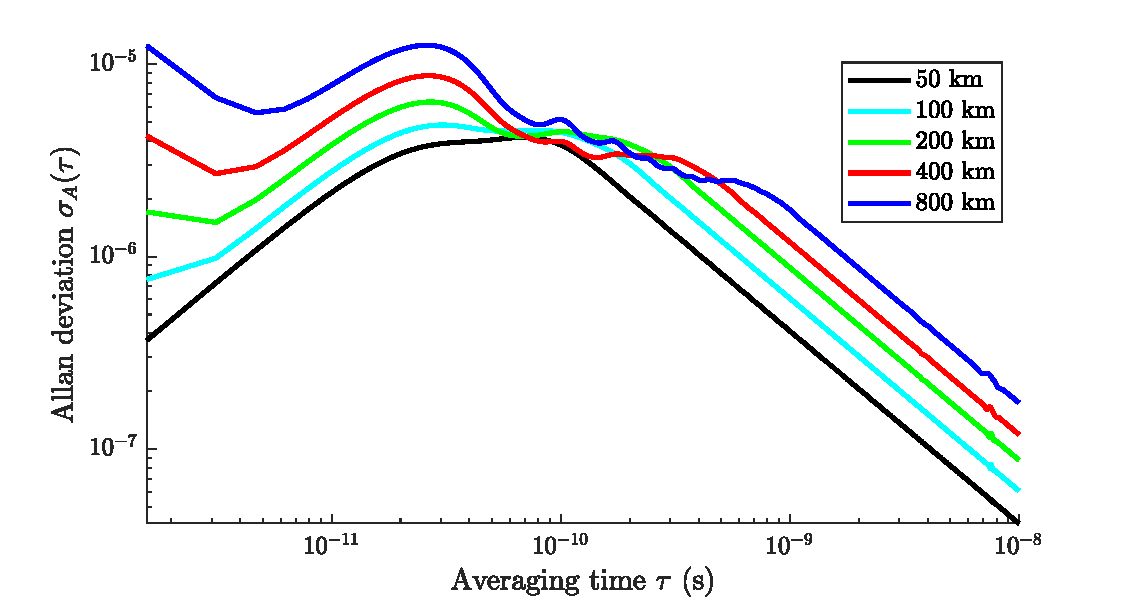
\includegraphics{img/AAllanDev}
	\caption{Allan Deviation with attenuation} \label{fig:AAllanDev}
\end{figure}
%
Finally, the Allan Deviation will be comparable to the results in the previous section. Figure~\ref{fig:AAllanDev} shows the Allan Deviation for several fiber lengths, the bump at the early time intervals corresponds with larger short term frequency errors, but they are averaged out very quickly and, once again, there are no long term frequency errors. The Allan Deviation will continue at a rate of $\tau^{-1}$. At $\tau=1$ s ADEV $=10^{-15}$, and at $\tau=10^3$ s ADEV $=10^{-18}$.


\section{Varying the Group Velocity Difference}

The relative group velocity difference governs the rate that a bit pulse will travel through a fixed time point. The group velocity difference is related to the separation between the center frequencies of the data and frequency channel. The value $d = 1.003$ ps/km was chosen because it corresponds with the greatest group velocity difference while adhering to the ITU grid standard. As the distance between the center frequencies decreases, the group velocity difference increases. Figure~\ref{fig:GVPhaseStability} shows the phase stability for different group velocity differences. 
%
\begin{figure}[htb]
	\centering
	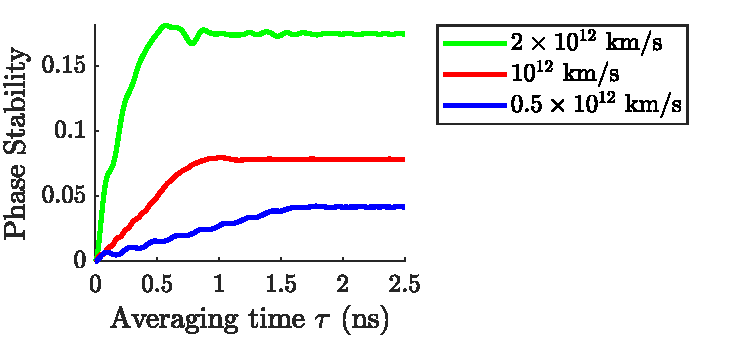
\includegraphics{img/GVPhaseStability}
	\caption{Phase stability vs. group velocity difference} \label{fig:GVPhaseStability}
\end{figure}
%



\section{Chapter Remarks}

Since the bits of any data channel are uncorrelated, the phase stability will asymptote at an averaging time corresponding to the duration of a bit window and the relative group velocity of the data channel. When the relative group velocity is greater, the asymptote occurs sooner because the data channel passes through a fixed time point at a much greater rate. 

The Allan Deviation represents the amount of frequency error. Experiments performing frequency transfer with a frequency signal and data channel located on the ITU standards have Allan Deviation values comparable to our simulated values \cite{Serrano2013} \cite{cantin2017progress}. The source of error in the experiments is due to temperature. So we see that moving the frequency signal in the interstices of two data channels gives a frequency error on the order of environmental effects.